\documentclass{article}
\usepackage[utf8]{inputenc}
\usepackage{blindtext}
\usepackage{amssymb}
\usepackage{setspace}
\usepackage{lipsum}
\usepackage{hyperref}
\usepackage{amsmath}
\usepackage[english]{babel}
\usepackage{amsthm}
\newtheorem{theorem}{Theorem}
\usepackage{algpseudocode}
\usepackage{algorithm}
\usepackage{graphicx}
\newtheorem{lemma}[theorem]{Lemma}
\usepackage{listings}

\title{COMP 550 – Algorithms and Analysis}
\author{Spring 2023-Assignment06}
\date{  Issue Date: April 10, 2023 
        $\vspace{0.5cm}$
        \\Due Date: Monday, April 17, 11:55 pm
        $\vspace{0.5cm}$
        \\ Marks: 5
        \\
        $\vspace{1cm}$
        \\ Student Name:$\rule[-5pt]{8.2cm}{0.05em}$ 
        $\vspace{1cm}$
        \\ Student PID:$\rule[-5pt]{8.2cm}{0.05em}$ }

\begin{document}

\maketitle
\begin{center}
\textbf{Submission:}
\end{center}
\begin{itemize}
    \item \textbf{You must upload your submission(s) before the deadline in Gradescope.}
    \item \textbf{Please ensure that your answers are within the given space allocated after the question.}
\end{itemize}

$\vspace{0.2cm}$

\begin{center}
\textbf{Rules for ALL HWs}:
\end{center}
You are encouraged to \textit{\underline{\textbf{discuss}}} the homework assignments and study together in groups, but when it comes to formulating/writing solutions \textit{\underline{\textbf{you must work}}} \textit{\underline{\textbf{alone and independently}}}. If required, you should be able to explain your answer clearly to TAs/LAs. Copying homework solutions from another student, from the  Internet, solution sets of friends, or other  sources will be considered cheating and treated accordingly.
\newpage

\section{Graph}
\doublespacing
\begin{enumerate}
    \item Let $G=(V,E)$ be an undirected, unweighted graph with $n=|V|$ vertices. The distance between two vertices $u,v \in G$ is the length of the shortest path between them. A vertex cut of $G$ is the subset $S \subseteq V$ such that removing the vertices in $S$ (as well as incident edges) disconnects G.\\
    Show that if there exists $u,v \in G$ of distance $d>1$ from each other, that there exists a vertex cut of size at most $\frac{n-2}{d-1}$. Assume $G$ is connected. 
    \newpage

    \item Run the Bellman-Ford algorithm on the following graph from source $A$. Relax edges $(U,V)$ in the lexicographic order, sorting first by $u$ then by $v$
    \\
    \
    \\
        \\
    \
    \\
    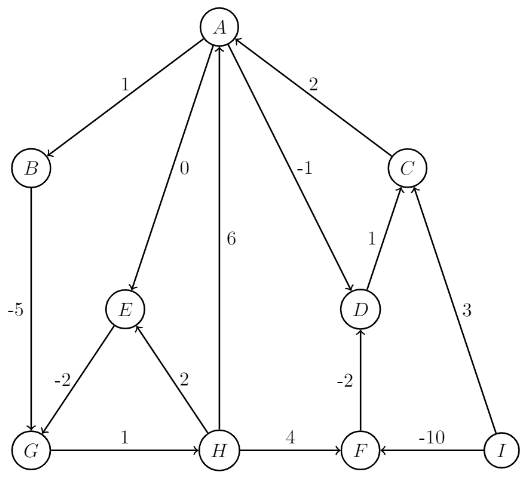
\includegraphics[scale=0.7]{image.png}
    \newpage
    \item For the graph in question 2, what problem occurs when we change the weight of edge $(H, A)$ to 1? How can we detect this problem when running Bellman-Ford? Why does this work?
    \newpage
\end{enumerate}

\section{Design algorithm}
\begin{enumerate}
    \item You have a computer and $n$ processes with the processing time $t_1,t_2,\dots t_n$. You have to pick the order in which to run the processes. Let $p_i$ denote the $i^{th}$ process you run. Then, the completion time $C_i$ for the process $p_i$ is defined as $C_{pi}=\sum_{j=1}^{i} t_{p_j}$ (the sum of times for all the processes up till this one ends). Design an algorithm and give its time complexity that minimizes the average completion time($\sum_{i=1}^{n} C_{p_i}$)
    \newpage
    
\end{enumerate}


\end{document}